\begin{figure}
    \centering
    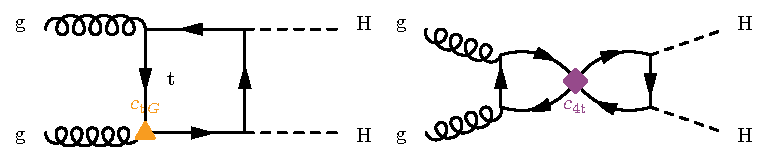
\includegraphics[width=\textwidth]{Diagrams/pdf/subleading}
    \caption{Representative Feynman diagrams induced by the subleading dimension-6 operators of Eq.~\eqref{eq:smeftL}~\cite{DiNoi:2024fdz}. Left: the chromomagnetic operator $c_{\PQt G}$ modifies the top--gluon vertex, marked by the triangle. Right: the four-fermion operators, collectively denoted $c_{4\PQt}$ and comprising $c_{Q\PQt}^{(1)}$, $c_{Q\PQt}^{(8)}$, $c_{QQ\PQt\PQt}$ and $c_{QQ}^{(8)}$, enter through the contact interaction between two top-quark loops, marked by the diamond. Unlike the leading operators of Fig.~\ref{fig:feymnhh}, none of the subleading operators can be mapped onto a HEFT coupling: they act on the top--gluon vertex and through additional top-quark loops, neither of which has an analogue in the five-operator HEFT set. The HEFT colour coding is therefore not carried over to this figure.}
    \label{fig:feymnhh_subleading}
\end{figure}
